\section{Collimator\_radial: A radial Soller blade collimator}
\index{Optics!Radial collimator}

\component{Collimator\_radial}{(System) E.Farhi, ILL}{$w_1$, $h_1$, $w_2$, $h_2$, $len$, $\theta_{min}$, $\theta_{max}$, $nchan$, $radius$}{$divergence$, $nblades$, $roc$ and others}{Validated}

\begin{figure}
  \begin{center}
    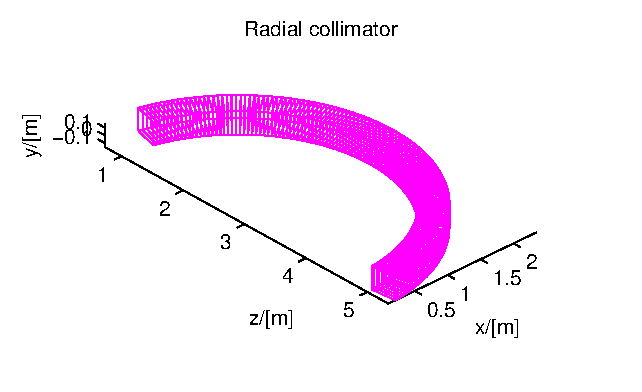
\includegraphics[width=0.8\textwidth]{figures/radial.eps}
  \end{center}
\caption{A radial collimator}
\label{f:coll-radial}
\end{figure}

This radial collimator works either using an analytical approximation
like {\bf Collimator\_linear} (see section \ref{collimator-linear}),
or with an exact model.

The input parameters are the inner radius $radius$, the radial length $len$,
the input and output window dimensions $w_1$, $h_1$, $w_2$, $h_2$,
the number of Soller channels $nchan$
(each of them being a single linear collimator) covering the angular interval
[$\theta_{min}$, $\theta_{max}$] angle with respect to the $z$-axis.

If the $divergence$ parameter is defined,
the approximation level is used as in {\rm Collimator\_linear}
(see section \ref{collimator-linear}).
On the other hand, if you perfer to describe exactly the number of blades
$nblades$ assembled to build a single collimator channel,
then the model is exact, and traces the neutron trajectory inside each Soller.
The computing efficiency is then lowered by a factor 2.

The component can be made oscillating with an amplitude of $roc$ times
$\pm w_1$, which supresses the channels shadow.

As an alternative, you may use the {\bf Exact\_radial\_coll} contributed component.
For a rectangular shaped collimator, instead of cylindrical/radial, you may use the Guide\_channeled and the Guide\_gravity components.
